\chapter{Analyse des opportunités des technologies libres dans le
domaine de l'édition vidéo et prévisions}

\minitoc \newpage

\paragraph{}

Maintenant que les besoins et que les solutions existantes ont été
analysées on rendra compte de la situation actuelle des technologies
libres et de leurs communautés. Il est aussi important de chercher
les raisons qui expliquent que ces logiciels ne sont pas plus utilisés
par les professionnels. Puis, nous essayerons d'envisager les solutions
possibles qui permettraient de remédier à cette situation.

\paragraph{}

Dans cette partie, nous analyserons la différence entre les manières
d'envisager la création de logiciel et nous verrons quels sont les
avantages et inconvénients de ces fonctionnements. Par la suite nous
nous concentrerons sur les frameworks existants pour faire une analyse
technique des ces technologies. Puis, nous analyserons les communautés
qui portent ces différents projets afin d'arriver à voir les lacunes
et les avantages de chacun des projets.  Pour finir, nous tirerons les
conclusions de cette analyse afin de trouver des solutions aux défis
qu'est la création d'un logiciel libre de montage vidéo.

\newpage

\section {Etat actuel de l'offre de logiciel libre}

Le schéma suivant permet de résumer facilement la situation:

\begin{figure} [h]
  \begin{center}
    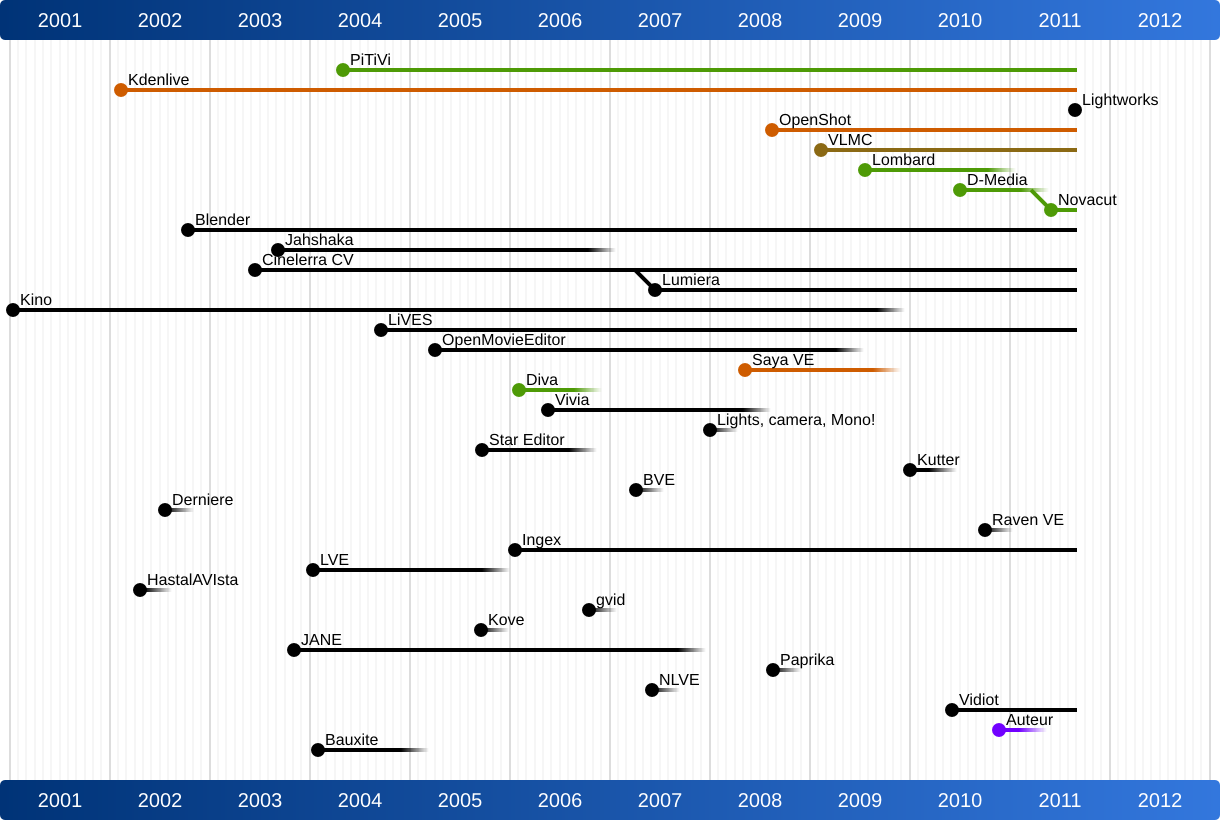
\includegraphics[width=0.9\textwidth]{images/open-source-video-editor-timeline}
  \end{center} \caption{Open source video editors timeline (Auteur:
  Jean-François Fortin, PiTiVi designer)} \label{Yes}
\end{figure}

\paragraph{ }

On constate donc que de nombreux projets de logiciel libre de montage
vidéo on vu le jours ces 10 dernières années, ayant différents
objectifs.  On peu distinguer deux types de public visés par ces projets:

\begin {itemize}

  \item {Les amateurs}

  \item {Les professionnels ou semi-professionnels}
\end {itemize}

\paragraph {Les amateurs de montages vidéo}

\subparagraph{}

Plusieurs projets libres permettent ou visent à répondre aux besoins
des amateurs, mais à l'heure actuelle ce cas d'utilisation n'est, dans
de nombreux cas, pas pleinement satisfait par les logiciels libres. Parmi
les logiciels dont l'objectif est de permettre de créer des montages
simples on distingue:

\begin {itemize}

  \item {openshot: Logiciel présentant  de nombreuses fonctionnalités,
  mais dont la
    qualité d'implémentation présente des faiblesses.}

  \item {kino: Logiciel avec un nombre de fonctionnalités limité
  permettant de faire des
    petit montages éfficacement}

  \item {Vidiot qui vise la production de vidéo amateur simple}

\end {itemize}

\paragraph {}

Mais les logiciels ayant pour objectif de pourvoir aux besoins plus
avancés en particulier à ceux des professionnels (précédemment
présenté dans le cadre de la définition des plus grands acteur du
marché) peuvent être utilisés dans le cadre de montage amateur. Bien
que leur utilisation, en particulier dans le cas du logiciel Cinelerra,
soit complexe.

\paragraph{}

Un nouveau projet a aussi récemment vu le jour, dont la finalité est
assez différente des logiciels actuellement présents. Il s'agit de
Novacut, qui permet aux créateurs de films et séries web de faire le
montage de manière collaborative à travers d'Internet, en partageant
les ressources (footage).

\paragraph{}

% Human readable version:

% Le fait que Cinelerra ne soit packagé dans aucune distribution

% Linux montre que même ce logiciel est le seul à avoir réussi à

% prendre une part de marché dans le milieu de l'édition

% professionnel, celui-ci n'a pas réussi à rassembler les

% développeurs et utilisateurs standard de logiciel libre.

Le fait que Cinelerra ne soit packagé \footnote{Packagé: fait
que qu'un paquet, une archive (fichier compressé) comprenant les
fichiers informatiques, les informations et procédures nécessaires
à l'installation d'un logiciel sur un système d'exploitation au sein
d'un agrégat logiciel, en s'assurant de la cohérence fonctionnelle
du système ainsi modifié est été créé. Source: Wikipedia} dans
aucune distribution Linux \footnote {Une distribution Linux, appelée
aussi distribution GNU/Linux pour faire référence aux logiciels du
projet GNU, est un ensemble cohérent de logiciels, la plupart étant
logiciels libres, assemblés autour du noyau Linux. Source: Wikipedia}.
montre que même ce logiciel est le seul à avoir réussi à prendre une
part de marché dans le milieu de l'édition professionnel, celui-ci n'a
pas réussi à rassembler les développeurs et utilisateurs standard de
logiciel libre.

\paragraph{}

En définitive aucun projet n'a encore réussi à s'imposer et ainsi
regrouper les développeurs au sein de projets majeurs. Dans d'autre
domaines, cela a été le cas, par exemple dans le domaine des lecteurs
vidéo, Vlc a su surpasser ses concurrents, et ainsi supplanter le
marché des lecteurs vidéo, qu'il soit libre ou non. Dans le domaine
des environnements de Bureau graphique, KDE et Gnome sont arrivés à un
stade où leur supériorité technique, et en terme de fonctionnalités,
fait d'eux des plateformes de référence.

\paragraph{}

Il est donc intéressant de se demander quelles technologies et quels
logiciel(s), pourraient se voir attribuer cette place dans le monde
de l'édition vidéo libre. Nous allons donc analyser les logiciels et
les technologies libres les plus avancés, (précédemment mentionnés
dans le cadre de l'analyse de marché: Cinelerra, Kdenlive et PiTiVi).
Nous verrons ainsi s'ils ont le potentiel de pouvoir un jour rivaliser
avec les logiciels propriétaires sur le marché très fermé du montage
vidéo professionnel.

\paragraph{}

NB: Il aurait été intéressant d'analyser le logiciel lightworks,
en voie de libération, mais à l'heure actuelle, aucun code n'a été
libéré, et par conséquent, celui-ci ne peut pas faire partie de
cette analyse.

\newpage

\section{Technologies}

\paragraph{}

Pour faire une analyse technique des produits permettant de faire
de l'édition vidéo, il est nécessaire d'analyser le ``core'' des
logiciels, c'est à dire la partie du logiciel où les opérations
d'édition sont effectivement réalisées. Dans ces domaines, il existe
deux façon de procéder:

\begin{itemize} \setlength{\itemsep}{2mm}

  \item{Création d'un logiciel monolithique\index{monolithique}}

  \item{Création d'un framework \glossary {name={framework},
   description={Un framework est un ensemble d'outils et de composants
   logiciels organisés conformément à un plan d'architecture et des
   designs patterns (un patron de conception, motif de conception ou
   modèle de conception est un concept de génie logiciel destiné à
   résoudre les problèmes récurrents suivant le paradigme objet.)}}
   \index{framework}}

\end{itemize}

\subsection {Technologies monolithiques\index{monolithique} VS
technologies modulaires, frameworks}


\subsubsection{Logiciels monolithiques \index{monolithique}} %FIXME Look
                                                             %for a def

\paragraph{}

Le conception monolithique \index{monolithique} dans le cadre des
logiciels d'édition vidéo, consiste à développer au sein d'un même
entité de code:

\begin{itemize} \setlength{\itemsep}{2mm}

  \item {la partie graphique et la partie de calculs
    permettant la gestion de tout ce que l'édition non linéaire
    implique}

  \item {L'interface utilisateur.}

\end {itemize}

\paragraph{}

Par le terme logiciel monolithique\index{monolithique}, il faut réaliser
que le logiciel peut utiliser des librairies externes, mais le core de
ce même logiciel, et la logique d'édition linéaire à proprement
parler sont directement faits à l'intérieur du logiciel et non par
une librairie ou framework \index{framework} externe. Cela a pour
principal avantage de présenter une conception simplifiée pour les
raisons suivantes:

\paragraph{}

Les logiciels professionnels (commerciaux) utilisent très probablement
tout ce mode de fonctionnement (même si probablement, en interne il ont
un core qui ressemble fortement à un framework \index{framework}).dans
le monde des logiciels libres,les développeures de Cinelerra ont décidé
d'utiliser ce mode de fonctionnement.

On peut voir plusieurs conséquences immédiates de ce mode de
développement:

\begin{itemize} \setlength{\itemsep}{2mm}

  \item {Les développeurs n'ont pas la nécessité de penser
    en terme d'interface publique de programmation (API\index{API}), et
    n'ont pas à garantir la stabilité de celle-ci: le risque réside
    dans le fait que la qualité de l'architecture ne soit pas optimale
    car la création d'API\index{API} oblige les développeurs/architectes
    à réellement analyser les besoins de manière plus large dès
    le début de la conception. Dans le cas où l'on ne crée pas
    d'interface publique de programmation vouée à être réutilisée,
    le risque est que le travail de design et d'architecture ne soit
    pas réalisé, et que le code grandisse de manière anarchique avec
    les différents développeurs qui font des extensions au fur et à
    mesure de leurs besoins.}

  \item {Les développeurs n'ont besoin de penser l'architecture seulement
  pour les cas d'utilisation qui sont liés à ce même logiciel:
    ils n'ont pas à voir au delà de ces use cases.}

  \item {Les erreurs en terme de design n'ont pas d'incidences aussi
    graves que dans le cas d'un framework\index{framework}.}
\end {itemize}

\paragraph{}

On se rend compte que cette manière de faire a pour principal avantage
le fait que le logiciel peut être développé plus rapidement puisque
le core du logiciel, et donc le code qui implémente la logique de
l'édition non linéaire, est conçue avec pour seul cas d'utilisation,
celui du logiciel. Cependant, de nombreux inconvénients existent à
cause de la nature monolithique\index{monolithique} du design:

\subparagraph{Besoins en main d'oeuvre considérables:}

\subparagraph { }

Dans le cadre de logiciel d'édition vidéo, le code à produire est
considérable, comme le montre les statistiques (Annexes 2). Le logiciel
Cinelerra à lui seul fait plus d'un million de lignes. Une telle
quantité de code est difficile à maintenir et requiert des ressources
importantes en terme de main d'oeuvre. Le fait que le logiciel soit
monolithique\index{monolithique} implique que celui-ci va être utilisé
seulement par ce logiciel, et par conséquent, les développeurs ne
peuvent pas compter sur d'autre utilisation de ce code pour améliorer
et développer le core du logiciel.

\paragraph{Réutilisabilité:}

\subparagraph { }

L'un des inconvénients de cette manière de faire est que le code que
l'on a à l'intérieur du logiciel n'est pas réutilisable directement
par d'autres projets, et par conséquent, on peut considérer que cela
est ``individualiste``, chose qu'il convient d'éviter dans le cadre du
développement de logiciel libre afin de ne pas multiplier les efforts,
et dupliquer le code.

\paragraph{}

Cette façon de faire a été utilisée par le projet Cinelerra. Ce
logiciel est le plus avancé en terme de fonctionnalités que le
marché des logiciels libres de montage offre. On peut penser que son
architecture monolithique\index{monolithique} explique ce développement
plus abouti, bien qu'il y ait évidemment de nombreux autres facteurs qui
interviennent en particulier le fait que ce logiciel a été développé
par la société Heroine Virtual.

\subsubsection {Utilisation de  frameworks \index{framework}}

\paragraph{}

L'autre possibilité est de séparer en deux parties bien distinctes
l'implémentation de la logique de l'édition, lecture, encoding vidéo
(core logiciel), de la partie graphique, interaction avec l'utilisateur
final.

\paragraph {Le framework}

\subparagraph{}

La grande différence entre la conception monolithiques
\index{monolithique} et la création d'un framework \index{framework}
réside dans le le fait que dans le cadre d'un framework, on développe
une API \index{API} autour du core du logiciel. Cela résulte dans le
fait que le core est un programme (librairie) externe, réutilisable par
n'importe quel autre application.  On peut considérer que les avantages
des frameworks sont les inconvénients des applications monolithiques
\index{monolithique} et vice-versa. L'avantage principal des frameworks
sur une conception monolithique\index{monolithique} est la possibilité
de partager un même code à travers de multiples applications. Celà
permet de réunir les efforts au travers, dans notre cas précis, de
tout type d'application multimedia.

\subparagraph{}

Dans le cadre de l'édition vidéo, on peut encore distinguer deux
manière d'envisager son développement:

\begin {itemize}

  \item {Utiliser un framework multimedia généraliste, et créer les
  outils nécessaire
         au montage au dessus de celui-ci} %stupid french!\ldots On top
                                           %of it?

  \item {Créer un framework spécialement orienté montage vidéo}

\end {itemize}

\subparagraph{}

Dans le monde du logiciel libre, ces deux manières d'envisager le
développement d'un framework multimedia ont été abordées par les
deux projets de framework leader sur ce segment:

\begin {itemize}

  \item {MLT qui se définit comme étant un ``Framework multimedia design
    et développé pour le brodcasting télévisé.''}

  \item {Gstreamer qui se définit comme étant un ``framework multimédia
    basé sur la notion de pipeline ce qui lui permet de nombreux types
    d'applications multimedia tels que des lecteurs multimédia, des
    logiciels de broadcasting, des logiciel de montage vidéo\ldots''}

\end {itemize}

\subparagraph {}

Au dessus de ces frameworks, plusieurs applications (interfaces graphique)
de montage vidéo se sont développées.

\begin {itemize}

  \item {PiTiVi: utilise le Framework multimedia GStreamer}

  \item {Kdenlive openshot utilisent le framework\index{framework}
  orienté édition et broadcasting MLT.}

\end {itemize}

\paragraph {}

Dans le cadre des Frameworks, nous nous intéresserons en particulier
à l'analyse de ceux-ci puisque les notions relatives à l'édition
vidéo, et la gestion de toute la partie multimédia est réalisée
par ceux-ci. Les logiciels d'édition ne sont à priori que de simples
interfaces graphiques basées sur ces frameworks. Dans les faits,
l'implémentation actuel de PiTiVi n'est pas qu'un simple interface
graphique au dessus de GStreamer, mais une partie de la logique de la
logique d'édition vidéo est actuellement faite dans le logiciel même
(ceci est entrain de changer et la migration \cite{PitviPortToGes}
vers gstreamer-editing-services\cite{PresentationOfGes}).

\newpage \section{Analyse technique}

\paragraph {}

Dans cette partie nous allons analyser les entrailles des trois logiciels
précédemment définis: Cinelerra, PiTiVi et Kdenlive.

\subsection{Cinelerra:}

\subsubsection{Documentation du code}

\subparagraph{}

Au niveau de la documentation, celle-ci est inexistante et le code
lui même ne contient que très peu de commentaires. Il est donc très
compliqué de comprendre le fonctionnement et les relation entre ces
centaines de millier de ligne de code. L'analyse de son fonctionnement
est par conséquent assez complexe, et il est possible que cette analyse
contienne des incertitudes.

\subsubsection {Structuration du code}

En terme de structure, le code de Cinelerra est décomposé en 3 partie:

\begin{itemize}

  \item{Lecture, rendering  audio vidéo: ce code est principalement
    contenu dans les dossiers ``quicktime'', ``thirdparty'' et
    ``libmpeg3''.}

  \item{Effets audios et vidéos: Ceux-ci sont développé comme plugins,
    et le code est donc présent de le dossier ``plugins`` }

  \item{Edition vidéo non linéaire et interface graphique: ce code est
    contenu dans un seul et unique dossier, ``cinelerra''}

  \item{Système de plugins: Aussi développé dans le dossier
  ``cinelerra``}

\end{itemize}

\paragraph{}

Cette structure semble être assez limité puisqu'il convient en théorie
de décomposer le code par petites parties, alors que dans le cadre de
Cinelerra, le dossier ``cinelerra'' contient non  moins de 1000 fichiers
et 207789 lignes de code.

\subsubsection{Lecture, rendering}

\paragraph{}

Dans le cadre de la lecture audio et video, Cinelerra fait appelle à
diverse librairies:

\begin{itemize}

  \item{ffmpeg: Solution compete, cross plateforme
  d'enregistrement, lecture, conversion de flux audio et vidéo. Il
  inclue libavcodec, librairie leader dans le domaines des
  coder/decoder\glossary{name={codec}, description={Un codec est un
  procédé
capable de compresser et/ou de décompresser un signal numérique. Ce
procédé peut être un circuit imprimé ou un logiciel.}}\index{codec}.
Il s'agit du core de la
  lecture audio et vidéo de Cinelerra.}

  \item{faac/faad: AAC audio encoder/decoder}

  \item{x264: h264 encoder}

  \item{libdv: DV codec}

  \item{\ldots}

\end{itemize}

\subparagraph{}

Toutes ces librairies sont utilisées dans le but de lire et écrire des
fichiers multimedia. Afin de standardiser, et permettre l'utilisation de
ces libraries de manière similaire au sein du logiciel, les développeurs
de Cinelerra ont élaboré au cas par cas des pont entre ces librairies
et le reste du logiciel (Fichier dans le dossier quicktime).

\subparagraph{}

% humaine readable

%De plus, les créateurs de Cinelerra ont développer des librairies de

%codec\index{codec}, muxer et demuxer (En

%particulier Mpeg et quicktime) afin d'ameliorer l'utilisation des ces

%formats dans le cadre de l'édition vidéo. Celà à tout de même été

%effectué dans de librairies extern réutilisable par d'autre projet:

\begin{itemize}

% Human readable:

% Quicktime 4 Linux: supporte en particulier les format DV,

% les codecs H.264 et AAC, et implémente des éléments de conversion

% d'espaces colorimétrique (colorspace conversion)

  \item {Quicktime 4 Linux: supporte en particulier les format DV,
    les codecs H.264 et AAC, et implémente des éléments de conversion
    d'espaces colorimétrique \glossary {name={espace colorimétrique},
    description={Un espace colorimétrique ou espace de couleur associe
    des nombres aux couleurs visibles. Compte tenu des limites de la
    vision humaine, ces nombres se présentent généralement sous
    la forme de triplets. Chaque couleur de lumière peut donc être
    caractérisée par un point dans un espace à trois dimensions. Lors
    d'une impression, pour des raisons liées à la qualité des pigments,
    l'espace utilisé comporte alors généralement au moins quatre
    dimensions. Source: Wikipedia}} (colorspace conversion)}

% Human readable

% Libmepg3: supporte la plupart des format du ``Mpeg Picture

% Motion Group''  et permet l'édition vidéo en utilisant ces

% format bien que pas conçu pour ce cas d'utilisation.

  \item {Libmepg3: supporte la plupart des formats du ``Mpeg Picture
    Motion Group'' \glossary{name={mpeg}, description={MPEG, sigle de
    Moving Picture Experts Group, est le groupe de travail SC 29/WG 11
    du comité technique mixte JTC 1 de l’ISO et de la CEI pour les
    technologies de l’information. Ce groupe d’experts est chargé
    du développement de normes internationales pour la compression, la
    décompression, le traitement et le codage de la vidéo, de l’audio
    et de leur combinaison, de façon à satisfaire une large gamme
    d’applications. Source: Wikipedia}} et permet l'édition vidéo en
    utilisant ces format bien que pas conçu pour ce cas d'utilisation.}

\end{itemize}

\subsubsection {Effets audio et vidéo}

Afin de permettre la création d'effets, Cinelerra utilise du  code
provenant de deux librairies:

\begin{itemize}

  \item {ladspa, Linux Audio Developers Simple Plugins API: Librairie
  d'effets audios qui
    contient une multitude de plugins.}

  \item {frei0r: Framework minimalist multi platform de création
  d'effets vidéo,
    il permet la création d'effet à travers de plugins. Il s'agit du
    standard de fait en terme d'effets vidéo.}

\end{itemize}

\paragraph{}

Afin de permettre l'utilisation d'effets, les développeurs de Cinelerra
on mis en place un système de plugins. En terme d'implémentation,
Cinelerra reprend le code de ces librairie dans un set de plugins
Cinelerra en ajoutant l'implémentation de l'interface graphique qui
permet la configuration de ces effets.

\subsubsection{Interface Graphique}

\paragraph{}

L'interface graphique est développé en utilisant directement le server
X sans aucune librairie graphique au dessus. Celà a pour conséquence
d augmenté le code à produire mais permet de controller complètement
le projet sans dépendre de ces librairies.  Dans le cadre de Cinelerra,
cela est sensé puisque ce logiciel est développé quasi intégralement
en interne.

\begin{figure} [H]

  \begin{center}

    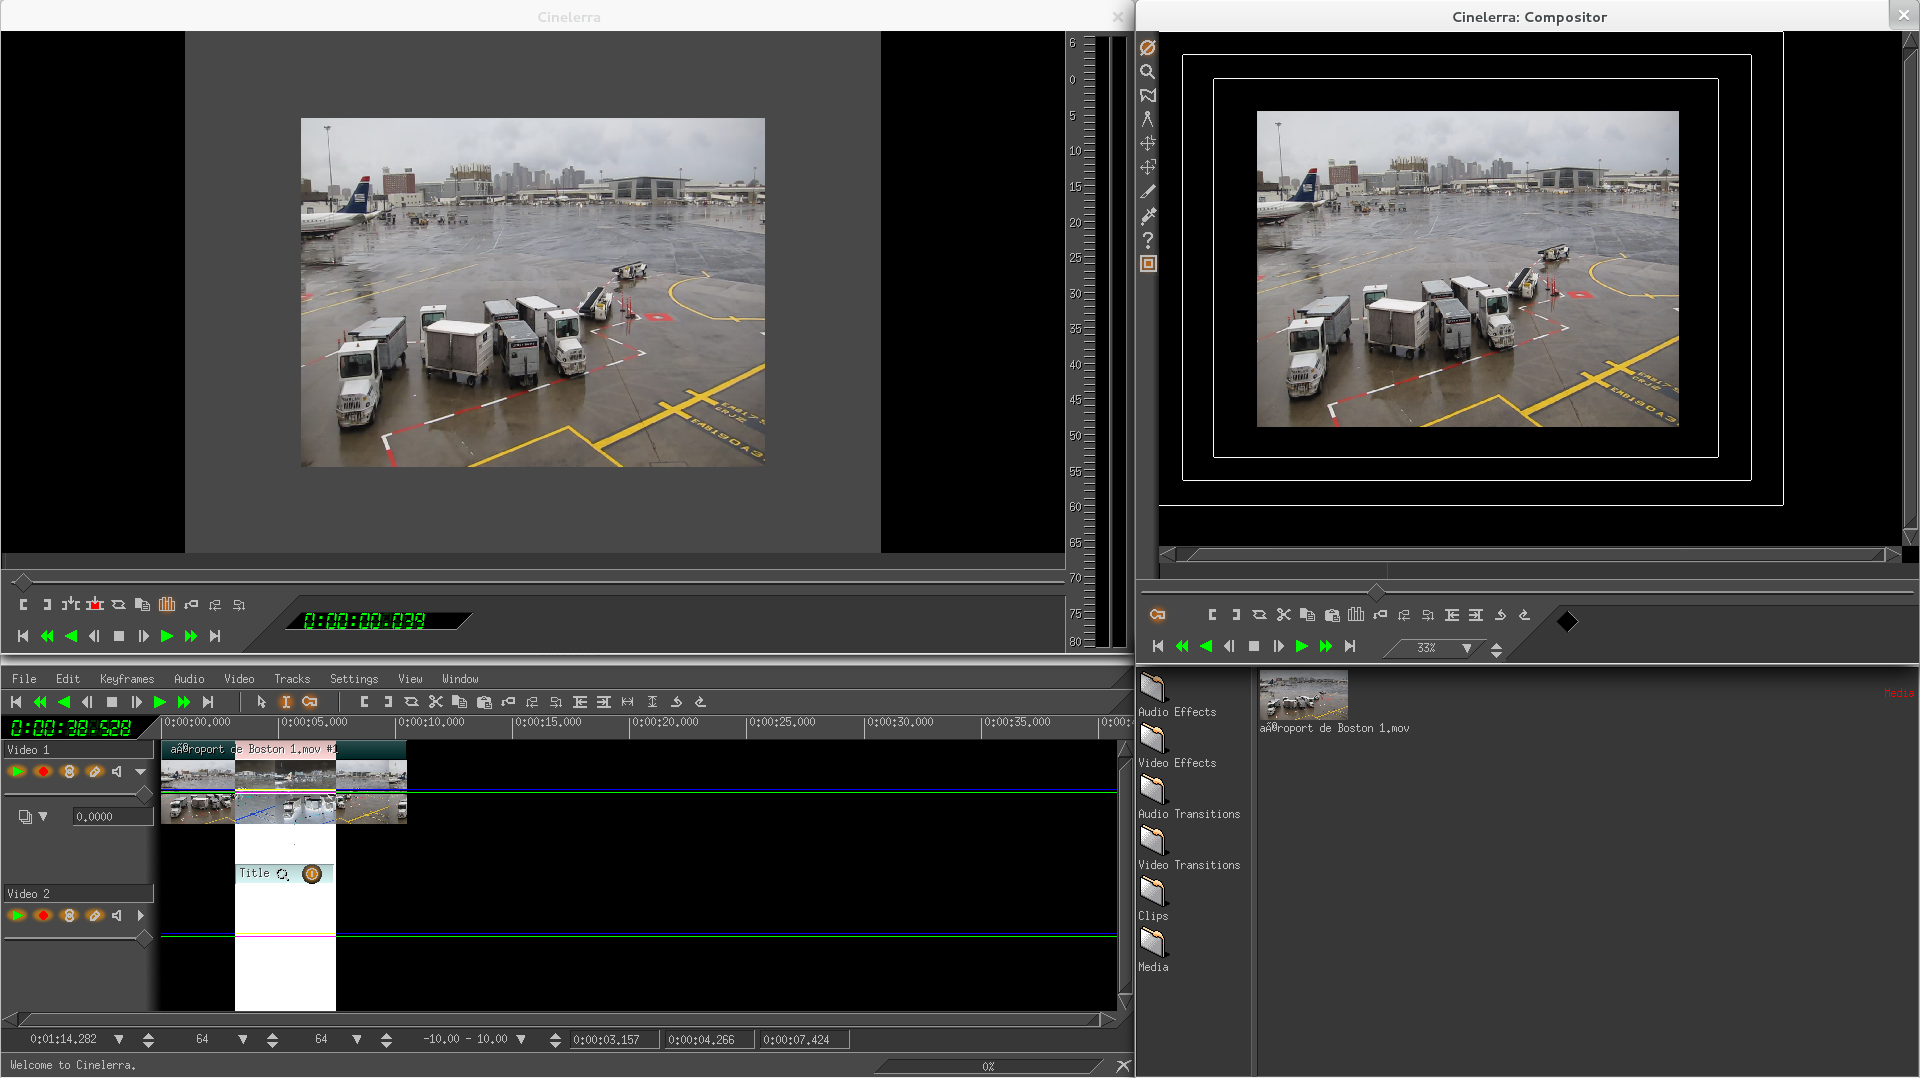
\includegraphics[width=0.95\textwidth]{images/cinelerra}

  \end{center}

  \caption{Interface graphique de cinelerra}

  \label{Yes}

\end{figure}

\paragraph{Structure de l'interface graphique:}

L'interface graphique de cinelerra est composé de quatre fenêtres
principales:

\begin{itemize}
  \item {La timeline (en bas à gauche sur le screenshot): cette
    partie permet de gérer un grand nombre d'action sur le contenu de
    la timeline.}

  \item {La fenêtre de ressource (un bas à droite sur le screenshot):
    dans, cette fenêtre, l'utilisateur peu accéder au différent
    footage qu'il a importer, il peut aussi accéder au différent effets,
    transitions\ldots}

  \item {Le fenêtre de preview (en haut à gauche sur le screenshot):
    cette fenêtre permet la prévisualisation des footage avant de les
    importer dans la timeline}

  \item {La fenêtre de composition (en haut à droite sur le screenshot):
    cette fenêtre permet d'effectuer des operation sur les vidéo et
    de prévisualiser la timeline.}

\end{itemize}

\subsubsection{Edition non linéaire}

\paragraph{Conception}

\subparagraph{}

Dans Cinelerra, l'interface utilisateur et la logique de l'édition
vidéo sont deux partie complètement interdépendante. Au sein du
code, il n'est pas possible de savoir quel partie est plutôt liée à
l'interface graphique et quel partie fait les calculs. Celà est due au
fait de sa conception monolithique, les développeurs n'ont pas pris la
peine de dissocier ces deux parties qui sont conceptuelement complètement
différente. On s'aperçoit en lisant le code que

\paragraph{Acceleration materiel}

\subparagraph{}

Lorsque openGL\index{openGL} est présent sur le système, Cinelerra
est en mesure de l'utiliser directement, dans la mesure où cette
fonctionnalité ai été activé lors de la compilation. Celà à pour
effet d'accélérer, principalement la fonction de compositing, mais
aussi la gestion des effets vidéo.

\subsection {Kdenlive}

Comme précedemment anoncé, Kdenlive utilise le framework orienté montage
et broadcasting MLT. Dans cette partit, nous allons dans un premier temps
analyser ce framework.

\subsubsection {Framework multimedia orienté montage: MLT}


\newpage \section{Analyse des communautés}

\newpage \section{Lacunes}

\newpage \section{Solutions possibles}
